\chapter{Численное решение задачи с учётом роста трещин автоГРП в длину} \label{ch3}

С помощью метода Ньютона проведено решение поставленной задачи.
Результаты моделирования представлены на рис. \ref{fig:results1}.
 
\begin{figure}[H] 
\center
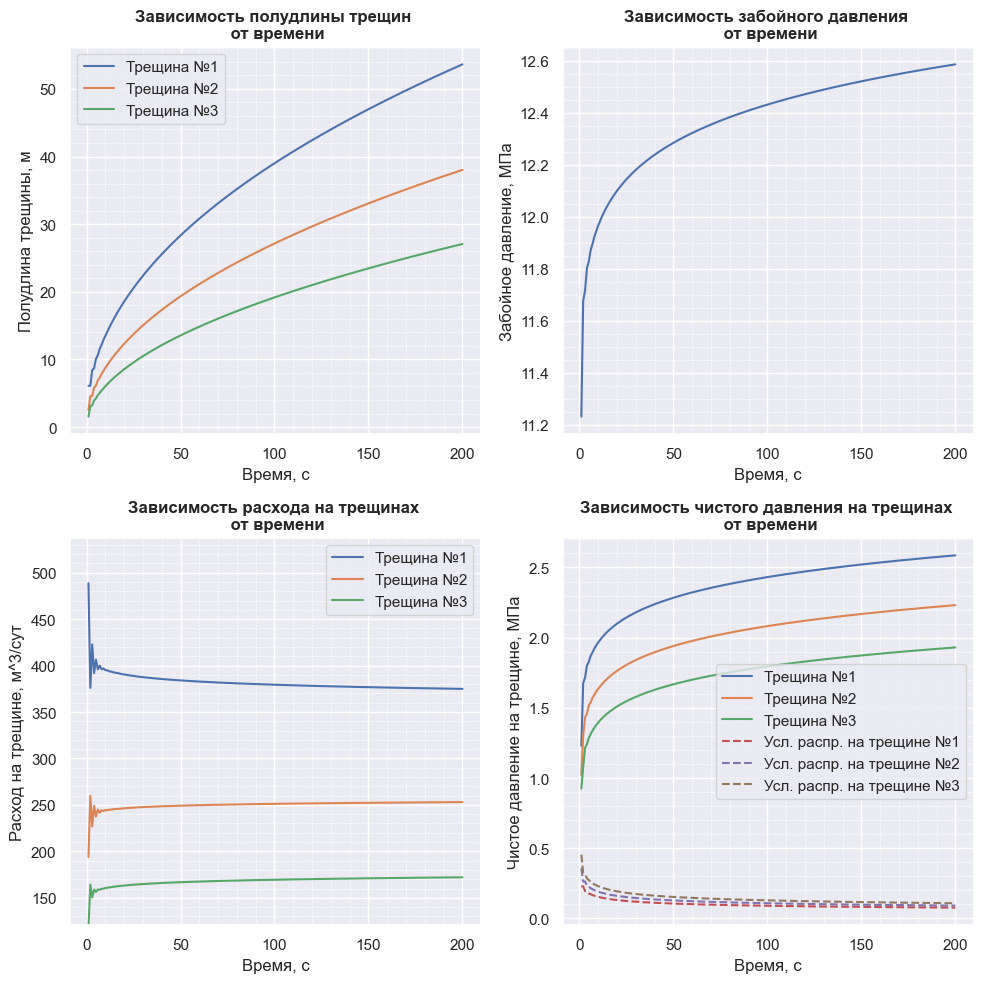
\includegraphics[width=0.9\linewidth]{images/Kirchhoff+Koning_1.png}
\caption{Результаты решения поставленной задачи при одновременном росте трёх трещин автоГРП} 
\label{fig:results1}  
\end{figure}

В проведённом численном эксперименте трещины отличаются друг от друга количеством и диаметром перфораций.\newline
У трещины 1: количество перфораций 32, диаметр перфораций 0.02 м.\newline
У трещины 2: количество перфораций 2, диаметр перфораций 0.01 м.\newline
У трещины 3: количество перфораций 1, диаметр перфораций 0.01 м.

Код решения представлен по ссылке: \url{https://github.com/mualal/hydrofracturing/blob/master/notebooks/03_fractures_growth_with_Koning_derivative.ipynb}.

Из графиков на рис. \ref{fig:results1} видим, что большую часть потока забирает на себя трещина с лучшими перфорациями.
Эта же трещина лидирует по скорости роста.

Также видим, что при росте трещин требуется всё большее забойное давление для того, чтобы поддерживать этот рост.

При выбранных входных параметрах построенной модели чистое давление в каждой из трещин существенно превышает давления критерия распространения, следовательно, при достаточно высоком забойном давлении все трещины будут расти одновременно.\\

\begin{figure}[H] 
\center
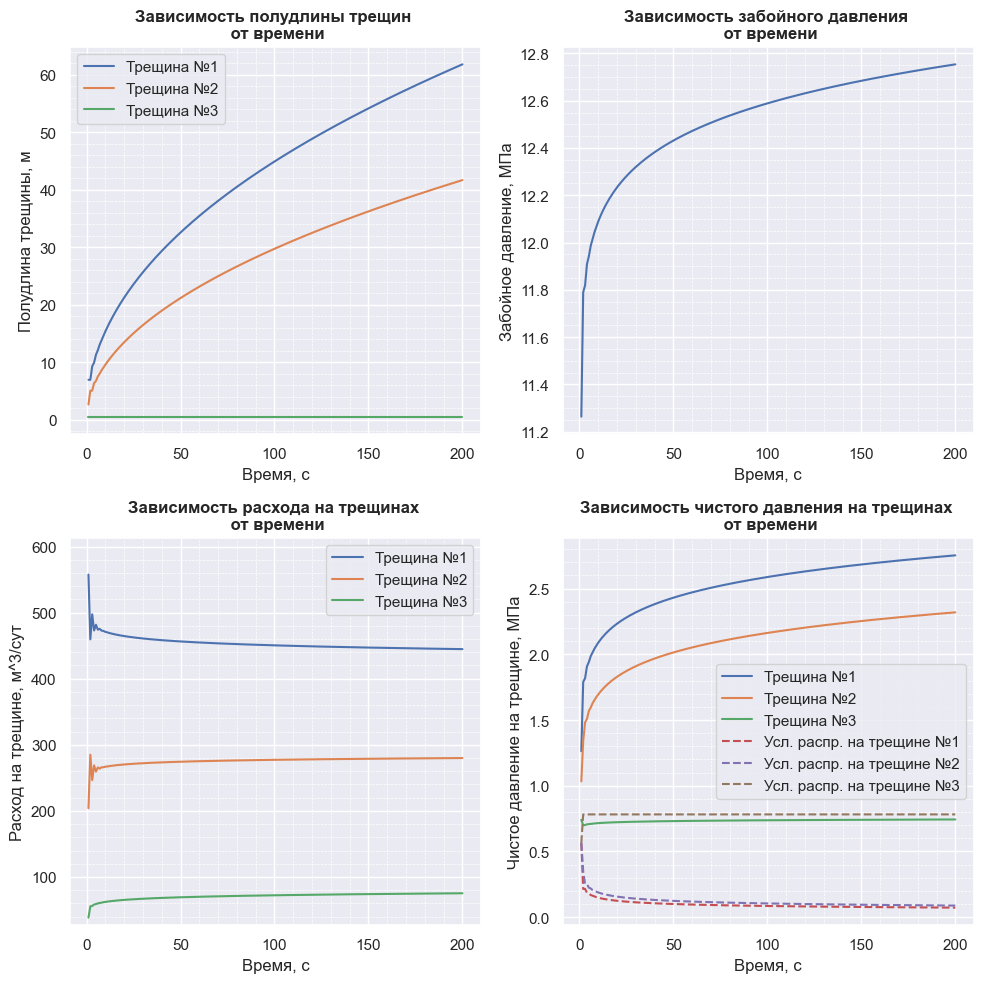
\includegraphics[width=0.9\linewidth]{images/Kirchhoff+Koning_2.png}
\caption{Результаты решения поставленной задачи при невыполнении критерия распространения на трещине №3} 
\label{fig:results2}  
\end{figure}

Далее проведено моделирование для случая с очень низким качеством перфораций на одной из трещин, при котором давление в этой трещине не превышает значение из критерия распространения.
Результаты представлены на рис. \ref{fig:results2}.

В проведённом численном эксперименте трещины отличаются друг от друга количеством и диаметром перфораций.\newline
У трещины 1: количество перфораций 32, диаметр перфораций 0.02 м.\newline
У трещины 2: количество перфораций 2, диаметр перфораций 0.01 м.\newline
У трещины 3: количество перфораций 1, диаметр перфораций 0.005 м.
\\

Также проведено моделирование в случае внезапного ухудшения качества перфораций на одной из трещин в момент времени $t_1=100\text{ с}$.
Результаты представлены на рис. \ref{fig:results3}.

\begin{figure}[H] 
\center
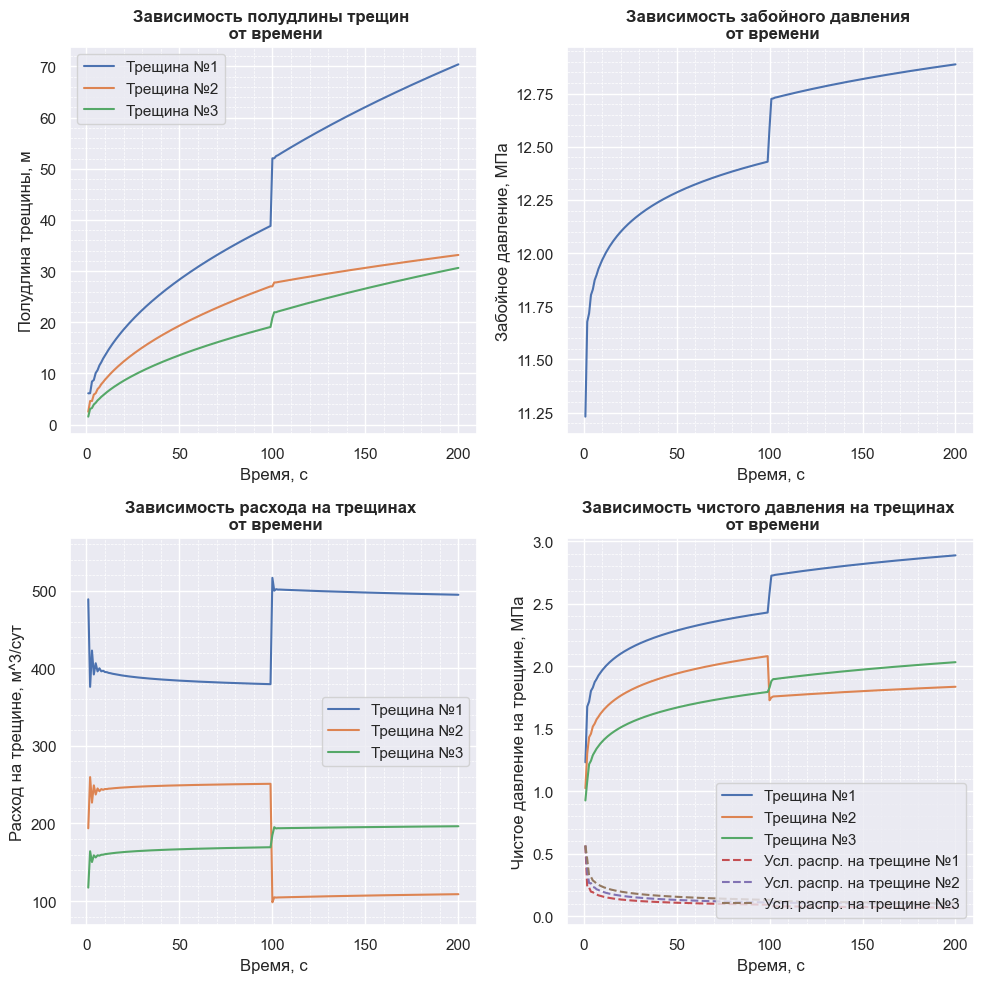
\includegraphics[width=0.85\linewidth]{images/Kirchhoff+Koning_3.png}
\caption{Результаты решения поставленной задачи при внезапном ухудшении качества перфораций на трещине №2 в момент времени $t_1=100\text{ с}$} 
\label{fig:results3}  
\end{figure}

Из проведённого численного эксперимента (рис. \ref{fig:results3}) видим, что внезапное ухудшение качества перфораций на одной из трещин автоГРП может негативно повлиять на эффективность эксплуатации месторождения, так как приводит к внезапному существенному росту длины соседних трещин при условии поддержания постоянного расхода на забое.\\

Для проверки работоспособности кода при большем количестве трещин автоГРП проведено моделирование в случае одновременного роста четырёх трещин.
Результаты представлены на рис. \ref{fig:results4}.

\begin{figure}[H] 
\center
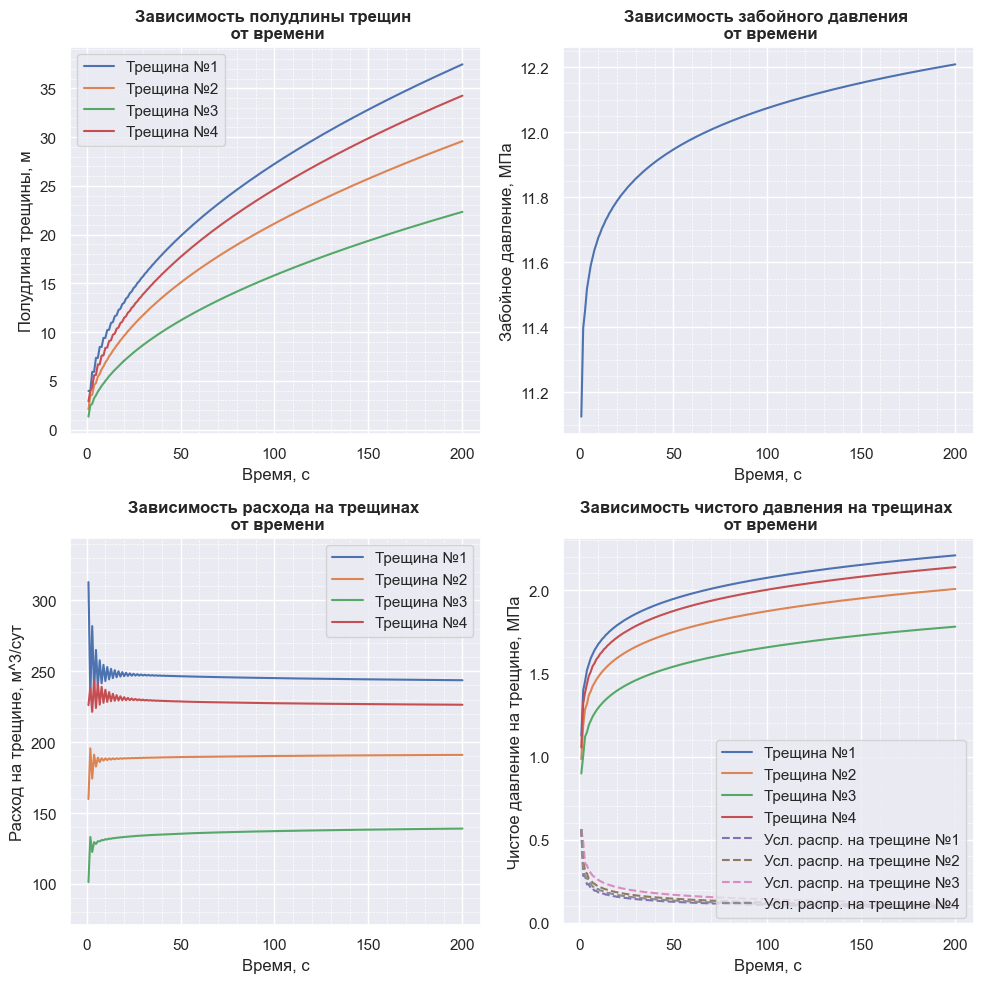
\includegraphics[width=0.85\linewidth]{images/Kirchhoff+Koning_4.png}
\caption{Результаты решения поставленной задачи при одновременном росте четырёх трещин автоГРП} 
\label{fig:results4}  
\end{figure}

